\section{Background}\label{sec:background}



\subsection{AUTOSAR}
%AUTOSAR (AUTomotive Open System ARchitecture) \cite{aa} is a collaborative project initiated by several large manufactures and suppliers in automotive industry to establish a shared standard for automotive E/E architectures. It is driven by the intention of getting better flexibility, scalability, reliability, and quality when the complexity of E/E system is greatly increasing. This kind of increased complexity is mainly concerned with the growth of the functional scope. Besides the goal of making the developers concentrate on the realization of the functionality rather than the design of the architectures, the standard of AUTOSAR also makes components developed by different manufacturers or software companies be able to be integrated with well-defined interfaces. 

%\subsubsection{AUTOSAR Abstraction}
AUTOSAR is a standard architecture to make vehicle software applications independent of the hardware. 
AUTOSAR also makes components developed by different manufacturers or software companies able to be integrated through well-defined interfaces.
Every AUTOSAR application is distributed to one or more Electronic Control Units (ECUs). 
An AUTOSAR software component is defined as the encapsulation of part of the functionality of the AUTOSAR application~\cite{aa}. An AUTOSAR application is composed of one or several SW-Cs. How to describe the interfaces of these AUTOSAR SW-Cs is defined and standardized within AUTOSAR. Each component can only be distributed to one AUTOSAR ECU. This is the reason why the AUTOSAR SW-C is called as ``Atomic Software Component"~\cite{aa}. AUTOSAR does not prescribe the size of the SW-Cs and how the SW-Cs are implemented. But in order to be able to  integrate several AUTOSAR SW-Cs correctly, one formal and complete description for one SW-C is needed when it is implemented. The description introduces how to configure the infrastructure for the component when building the system. 

Communication between AUTOSAR software components are conducted by well-defined ports. A port is  defined by an AUTOSAR interface. It can either be a {\em Provided Port} which provides data or a {\em Required Port} which receives data. There are two main types of communication patterns supported by AUTOSAR. One is {\em Client-Server} and another one is {\em Sender-Receiver}. In the {\em Client-Server} pattern, the client sends a request for service, the server performs the requested service, %after receiving it 
and then responds to the request. An AUTOSAR software component (SW-C) can be both a client and a server. The {\em Sender-Receiver} pattern realizes asynchronous communication. %A sender sends information to one or several receivers without receiving back an answer. 
The time and way to send back information are decided by the receivers.

Communication between different ECUs is performed with a shared virtual bus, which consists of hardware interfaces provided by the basic software in AUTOSAR infrastructure. The Runtime Environment (RTE) is an implementation of the Virtual Functional Bus (VFB). It provides a uniform environment for communication between components~\cite{aa}. In this way, when moving a component to another ECU, developers do not need to change any code of the component. %The layered architecture of the AUTOSAR software for an ECU is shown in Figure~\ref{fig:autosar}. 



This work focuses on the application layer which consists of application software components. %Examples of components in AUTOSAR applications are given. 
%However, in the following we provide a short description also of the other layers to enable a better understanding of how the system works. %  for better understanding of how the system runs, short descriptions of related concepts of others layers are also given.


%\subsubsection{AUTOSAR Software Component}
%AUTOSAR software component is defined as the encapsulation of part of the functionality of the AUTOSAR application~\cite{aa}. An AUTOSAR application is composed of one or several SW-Cs. How to describe the interfaces of these AUTOSAR SW-Cs is defined and standardized within AUTOSAR. Each component can only be distributed to one AUTOSAR ECU. This is the reason why the AUTOSAR SW-C is called as ``Atomic Software Component"~\cite{aa}. AUTOSAR does not prescribe the size of the SW-Cs and how the SW-Cs are implemented. But in order to be able to  integrate several AUTOSAR SW-Cs correctly, one formal and complete description for one SW-C is needed when it is implemented. The description introduces how to configure the infrastructure for the component when building the system. The introductions to the components that I work on are given below. 
%
%\noindent {\bf Brake-By-Wire Application} - In this paper we make use of 
%In order to better understand the functionality of the selected AUTOSAR software components in this thesis, the software application that includes these components should be introduced. Here is the Brake-By-Wire application. 
%
%The Brake-By-Wire application is a research framework developed by the DEDICATE project~\cite{pp} that implements a brake-by-wire function distributed over five ECUs. It is not the real system that is used in the real trucks. It is proposed to give a example of distributed safety-critical system for validating research projects. The BBW application also includes an environment model of the vehicle in order to simulate the behaviour of the entire vehicle with regards to acceleration and braking~\cite{pp}. When using this application, the Brake Pedal ECU gets the signal of braking, does calculation and then sends a corresponding brake force request to each wheel.
%
%\paragraph{Brake-Pedal-Input-Handler Component}
%The distribution of the Brake-Pedal-Input-Handler component in the Brake-By-Wire system is shown in Figure~\ref{fig:BPIH}. The function of this component is to convert the hardware pedal input into a pedal position (0-100\%). The input of this component is an integer with 12 bits and the output is a percentage from 0\% to 100\%. It provides input for the Brake-Torque-Calculation component and the Brake-Light-Control component.
%
%
%\begin{figure}[htb]
%\centering
%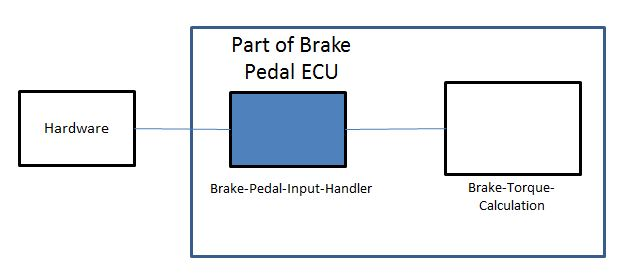
\includegraphics[width=\columnwidth]{figure/brakepedal1.jpg}
%\caption{Brake-Pedal-Input-Handler component distribution on ECU.}
%\label{fig:BPIH}
%\end{figure}
%
%\paragraph{Brake-Light-Control Component}
%
%The distribution of the SW-Cs in Brake-Lighting application is shown in Figure~\ref{fig:brakelighting}. The Brake-Light-Control Component is located on the BrakePedalECU. It inputs vehicle speed and brake pedal position (0-100\%) and outputs ON or OFF for the brake lights according to some rules. The basic rules~\cite{pp} are:
%
%\begin{enumerate}
%\item The brake light is always OFF when the pedal input is 0\%.
%\item The brake light is always fixed ON whenever the pedal input $>$ 0\% and the vehicle speed is $<$ 10km/h.
%\item From 10km/h and above the brake light will blink ON/OFF if emergency braking is active otherwise it is fixed ON.
%\end{enumerate}
%
%\begin{figure}[htb]
%\centering
%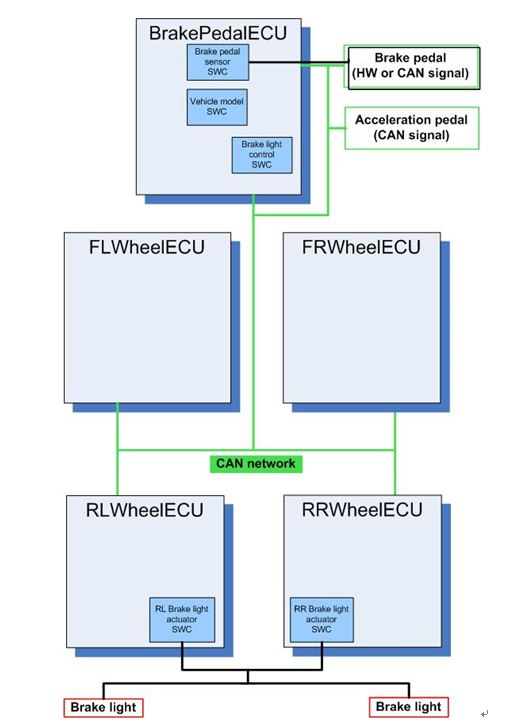
\includegraphics[width=.9\columnwidth]{figure/brakelighting.jpg}
%\caption{Brake lighting SW-Cs distribution on ECUs~\cite{pp}}
%\label{fig:brakelighting}
%\end{figure}

%
%\subsubsection{AUTOSAR Software Component Communication}
%Communication between AUTOSAR software components are conducted by well-defined ports. A port is  defined by an AUTOSAR interface. It can either be a Provider Port which provides data or a Required Port which requires data. There are two main types of communication patterns supported by AUTOSAR. One is Client-Server and another one is Sender-Receiver. In the Client-Server pattern, the client sends a request for service, the server performs the requested service, %after receiving it 
%and then responds to the request. An AUTOSAR software component (SW-C) can be both a client and a server. The Sender-Receiver pattern realizes asynchronous communication. A sender sends information to one or several receivers without receiving back an answer. The time and way to use the received information are decided by the receivers.
%%without getting a response from the receivers. And also, 
%%the time and way to use the received information are decided by the receivers. 

%\subsubsection{Virtual Functional Bus (VFB)}
%%The virtual functional bus (VFB)
%It is defined as the abstraction of the AUTOSAR SW-C interconnections~\cite{aa} on the vehicle. It enables the components on different ECUs to communicate with each other independent of the hardware and of which ECUs they locate. 

%\subsubsection{Runtime Environment (RTE)}
%%The runtime environment (RTE) 
%It is an information exchange center for communication inside one ECU or between different ECUs. It is the implementation of the VFB on a specific ECU~\cite{aa}. It provides the same interface for the SW-Cs to the AUTOSAR infrastructure and hardware despite where the SW-Cs are located. As different components are used in different applications, the RTE will be tailored in order to use resources more efficiently when the RTE is generated by the RTE generation tool. Sometimes, the RTE is tailored according to the configuration. All these make differences on the generated RTE of different ECUs. 
%
%\subsubsection{AUTOSAR Infrastructure}
%%The AUTOSAR infrastructure 
%It is a collection of basic software, which mainly consists of services, communication, operating system, ECU abstraction, microcontroller abstraction, and device drivers~\cite{aa}. Its function is to provide platform services to SW-Cs.


\subsection{Design By Contract}
Design by Contract, also known as programming by contract, is an approach for designing software, by which software can get better robustness. The key concept is ``viewing the relationship between a class and its clients as a formal agreement, expressing each party's right and obligations" \cite{jj}. The agreements are similar to the contracts in business. These contracts set conditions for input and output of software components. The conditions have three types, pre-condition, post-condition and invariant. When a client component calls an operation on a server component, the client component needs to meet the pre-condition which is specific for that operation. For the return of that operation, the requirements of the post-condition need to be meet, which is an obligation for the server component. Invariant is a certain property that are met for both of the two components. In this way, different components of a software system can collaborate with each other with high robustness. 

When Design by Contract was pioneered by Bertrand Meyer in the late 1980's, it was firstly used in the design of the Eiffel programming language~\cite{ii}. Later, this design philosophy of software started to be popular in languages with native support or with third-party support. 

%The following code~\cite{ii7} is a simple example of how Design by Contract works in C++. It is a short form of a class which omits some code not relevant to the example.
%
%\begin{figure}[htb]
%\centering
%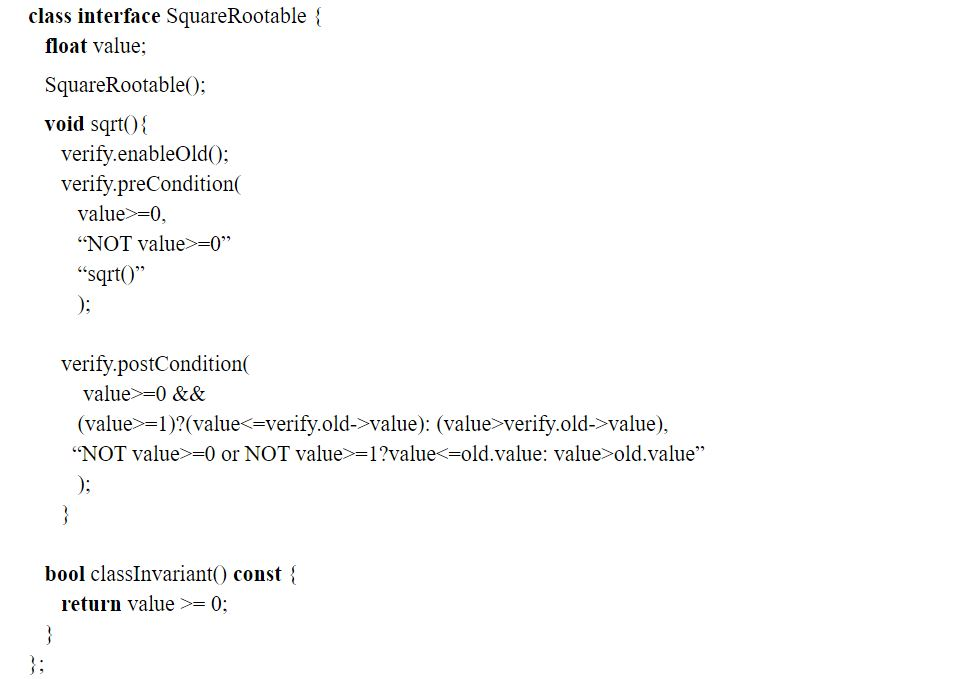
\includegraphics[width=0.9\linewidth]{figure/c++_code.jpg}
%\end{figure}
%
%This component functions as checking the input and output value of square root calculation. In this component, all the three types of conditions are set for the class. The pre-condition is that the input value should not be less than 0. The post-conditions are that the output value should be greater than 1 when the output value is less than the input value, and the output value should be greater than 0 and less than 1 when the output value is greater than the input value. The invariant for such a class is that the value should not be less than 0. If these criteria are not met, the calculation will not be conducted. This is a simple example for understanding such a design idea. 

In the C programming language, the application of Design by Contract is not obvious. % can be applied by assertions. 
For the reason that there are no classes in C, the subjects of the conditions are the functions. But the principles are similar. The caller function must meet all the preconditions of the callee function, and the callee function must meet its own post-conditions. The failure of either party of the contract is a bug in the software~\cite{jj}. Invariants in C are the conditions that must be hold for a structure or type\footnote{\url{http://www.onlamp.com/pub/a/onlamp/2004/10/28/design_by_contract_in_c.html}}. 

%When giving examples of setting conditions for software components in AUTOSAR, the conditions should derive from all the possible input (valid and invalid) and requirements specification. Using the Brake-Pedal-Input-Handler component as an example, the valid input is an integer from 0 to 4095 and the invalid input may be less than 0 or greater than 4095. The pre-condition can limit the input value in the valid range. Similarly, as the conversion calculation may make the output value less than 0\% or greater than 100\%. Obviously, the post-condition should check the output in the range of 0\%-100\%.

\subsection{Robustness}
Robustness is defined as ``the degree to which a system or component can function correctly in the presence of invalid inputs or stressful environmental conditions" in IEEE standard~\cite{cc}. The definition is similar to what is described in ISO 26262-1. The understanding of it is a bit different for software and hardware. For software, robustness is the ability to respond to abnormal inputs and conditions. For hardware, robustness is the ability to be immune to environmental stress and stable over the service life within design limits~\cite{bb}. 

In this paper we focus on the software part. Robustness of software refers to the capability of the %, on the one hand, good robustness means the 
system or component to %can 
(i) handle data correctly even when the input volume is very large, and (ii) %On the other hand, it should be able to 
handle invalid inputs to ensure the successful running of the system or component. As in the vehicle embedded system, most applications run repeatedly over a time period. The time period can be $5ms$, $10ms$ or $20ms$ according to the requirements of the application. %Considering the definition of Design by Contract, my work in this thesis mainly focuses on improving the capability of handling invalid inputs and ensuring valid outputs. That is how Design by Contract is applied.

The robustness of AUTOSAR software components is evaluated according to the rules described below:
\begin{itemize}
\item ARUnit (introduced in Section~\ref{sec:arunit}) is used to run black-box testing for the components. 
\item A list of data which may be valid or invalid is given as input to the component. 
\item For every input, the output can be data in the expected range, data outside the expected range, or error. 
\item Better robustness means more output data in the expected range, less output data outside the expected range and less errors. 
\item The comparison of them is used to benchmark the %shows the differences of different 
components' robustness.
\end{itemize}

 
\subsection{ARUnit}\label{sec:arunit}

ARUnit is a unit testing tool which provides a lightweight testing environment for AUTOSAR software components\footnote{\url{https://www.artop.org/arunit}}. It is based on Eclipse. After importing the components that need to be tested, it can compile the components and generate the run-time environment for each single AUTOSAR software component. %Of course, test cases can be defined in it as well for the reason that it provides an API to stimulate and query the state of the RTE from the outside. 
Test cases can be defined directly within the tool and moreover it provides an API to stimulate and query the state of the RTE from the outside. 
It is a quite convenient tool for operating unit testing effectively and efficiently. Figure~\ref{fig:ARUnit} shows how ARUnit generates RTE for AUTOSAR software components. %The way of how the data handled and exchanged inside  between component A and component B.

\begin{figure}[htb]
\centering
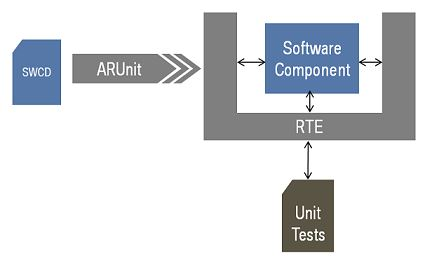
\includegraphics[width=0.9\linewidth]{figure/arunitin.jpg}
\caption{ARUnit provides RTE for single Software Component.}
\label{fig:ARUnit}
\end{figure}